\section{What is Heat?}

Heat is the project providing Orchestration for OpenStack. It allows cloud infrastructure to be represented in a declarative form (`template'). The Heat service parses these templates and calls the various OpenStack APIs to create or modify the deployment, while maintaining correct dependencies between them. The collection of resources associated with a template is known as a stack. One of the resource types available is a stack, so templates can be composed into hierarchical structures.

Heat provides equivalent functionality to the AWS CloudFormation service. CloudFormation templates are represented as \textsc{Json} documents referencing resources, and Heat is compatible with the CloudFormation template syntax (and a \textsc{Yaml} variant for easier consumption by humans).  Heat also provides a number of Cloudformation-compatible resource implementations, and a CloudFormation-compatible API.

Heat also provides a growing number of OpenStack native resource types, which aim to allow flexible and transparent configuration of the underlying OpenStack resources. Heat also has its own OpenStack-native \textsc{Rest} API, and work is in progress adding functionality to a native template language (Heat Orchestration Templates, aka "HOT").

\begin{figure}[h!]
\caption{Heat Overview Diagram}\label{HeatOverviewFigure}
\centering
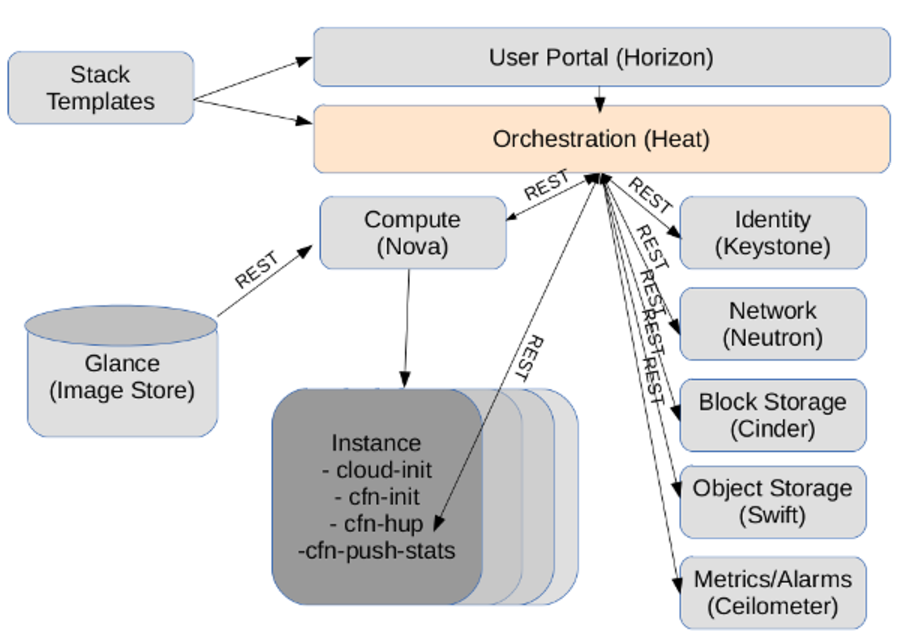
\includegraphics[scale=0.5]{images/heat-overview-diagram-small.pdf}
\end{figure}
